\section{Sprint 1: First iteration}
In this section, we will present and discuss the development that took place in the first iteration of our project. This includes a relevant presentation of the Scrum methodology as we have applied it in the sprint. We will mostly present artifacts created that are relevant to the inception and elaboration phases of the unified process.
\subsection{Scrum}
Scrum is an iterative framework designed to manage software development projects \cite{scrumguide} \\
The methods originally intends to include a team of up to eight persons, along with a Scrum Master and a Product Owner. However, as we were only five persons we had no choice but to appoint these roles to team members. Moreover, we decided that we wanted a more democratic approach to the features that we included in our project; this implied that the responsibility of creating product backlog items were spread out on the whole group instead of relying solely on the Product Owner \cite[p.~12]{scrumguide}.
\subsubsection{Initial Scrum}
Before initializing our first sprint, we decided to conduct two sprint planning meetings in somewhat extended versions. Since this were our first project in which we’ve used Scrum, we decided that we would ignore the time bounds that are specified in the Scrum guide \cite[p.~9]{scrumguide}. This allowed us to discuss and familiarize ourselves with the Scrum concepts.\\
The initial meetings were divided into several parts: First, we agreed on using the Scrumwise \cite{scrumwise} tool for organizing our Scrum activities. Then, we all democratically built the product backlog. \\
An important part of the formation of our team before the first sprint were also doing a formal written definition of done. This includes defining a strategy for testing, coding, documentation and acceptance from the rest of the team. The definition of done can be viewed in [section whatever: definition of done]\\
% add ref
Lastly, we had to agree on the number and length of the sprints we were going to do. This also meant creating an overall timeline of the sprints, which can be viewed in [Appendix Figur [sprinttimeline.jpeg]  These initial exercises allowed us to conduct the two, more formally defined meetings of sprint planning: part one of two, respectively. \\
A partial view of the product backlog can be found in Appendix, Figur \ref{backlog1}, page \pageref{backlog1} \\
%ref
\subsubsection{Sprint planning $|$ \& $\|$}
After our initial Scrum agreements, we conducted planning meeting part one for the next sprint. This involved several noteworthy items:
\begin{itemize}
\item Creating a capacity plan to get an overview of our initial work capacity [Appendix, Figur \ref{capacityplan}, page \pageref{capacityplan}]
%  ref
\item Estimating difficulty and priority of the items on the Product Backlog
\item And elaborating on the meanings of the different backlog items to each other (as part of not having a single product owner).
\end{itemize}
Then moving on to the second part of the meeting, where the team were:
\begin{itemize}
\item committing to highest prioritized tasks and estimating their time to complete
\item distributing the work so the workload was fair on each individual
\item initialize the sprint in the Scrumwise tool and review the burndown chart generated
\end{itemize}
An overview of the first Sprint Backlog is available in [Appendix, Figur \ref{sprint1backlog}, page \pageref{sprint1backlog}].\\
% ref
It is worth nothing that even though we decided on all having influence on the product backlog, the management of the backlog were deferred to one person, the “Product Owner”.\\
\subsubsection{More Scrum}
Our Scrum workflow also covers doing following exercises:\\
\begin{itemize}
\item Doing Daily Scrum meetings, updating burndown charts and reviewing our task boards
\item Updating our product backlog during the sprint so tasks are ready for next sprint
\item Doing the Scrum retrospective and review
\end{itemize}
However, we’ve chosen to defer the description and discussion of these exercises to later sprints where we think they’re more relevant.

\subsection{Initial Software Analysis}
This section will cover our initial analysis of the requirements as given in the project description [reference: project description]. We will describe different RUP artifacts created during the process, such as Use Cases, Domain Model, System Sequence Diagrams and Supplementary Requirements.\\
Please note that in the spirit of agile development, the artifacts created in the first sprints are incomplete and draft-like in appearance. The artifacts are then extended and reviewed in later iterations as the need for understanding them increases.\\
\subsubsection{Domain Model and Relational Model}
Before doing any design of the system, we realize the need for a common terminology to describe our understanding of file-sharing and document handling applications. We make a crude initial domain model in order to discuss our understanding of each entity:\\
\begin{figure}[H]
  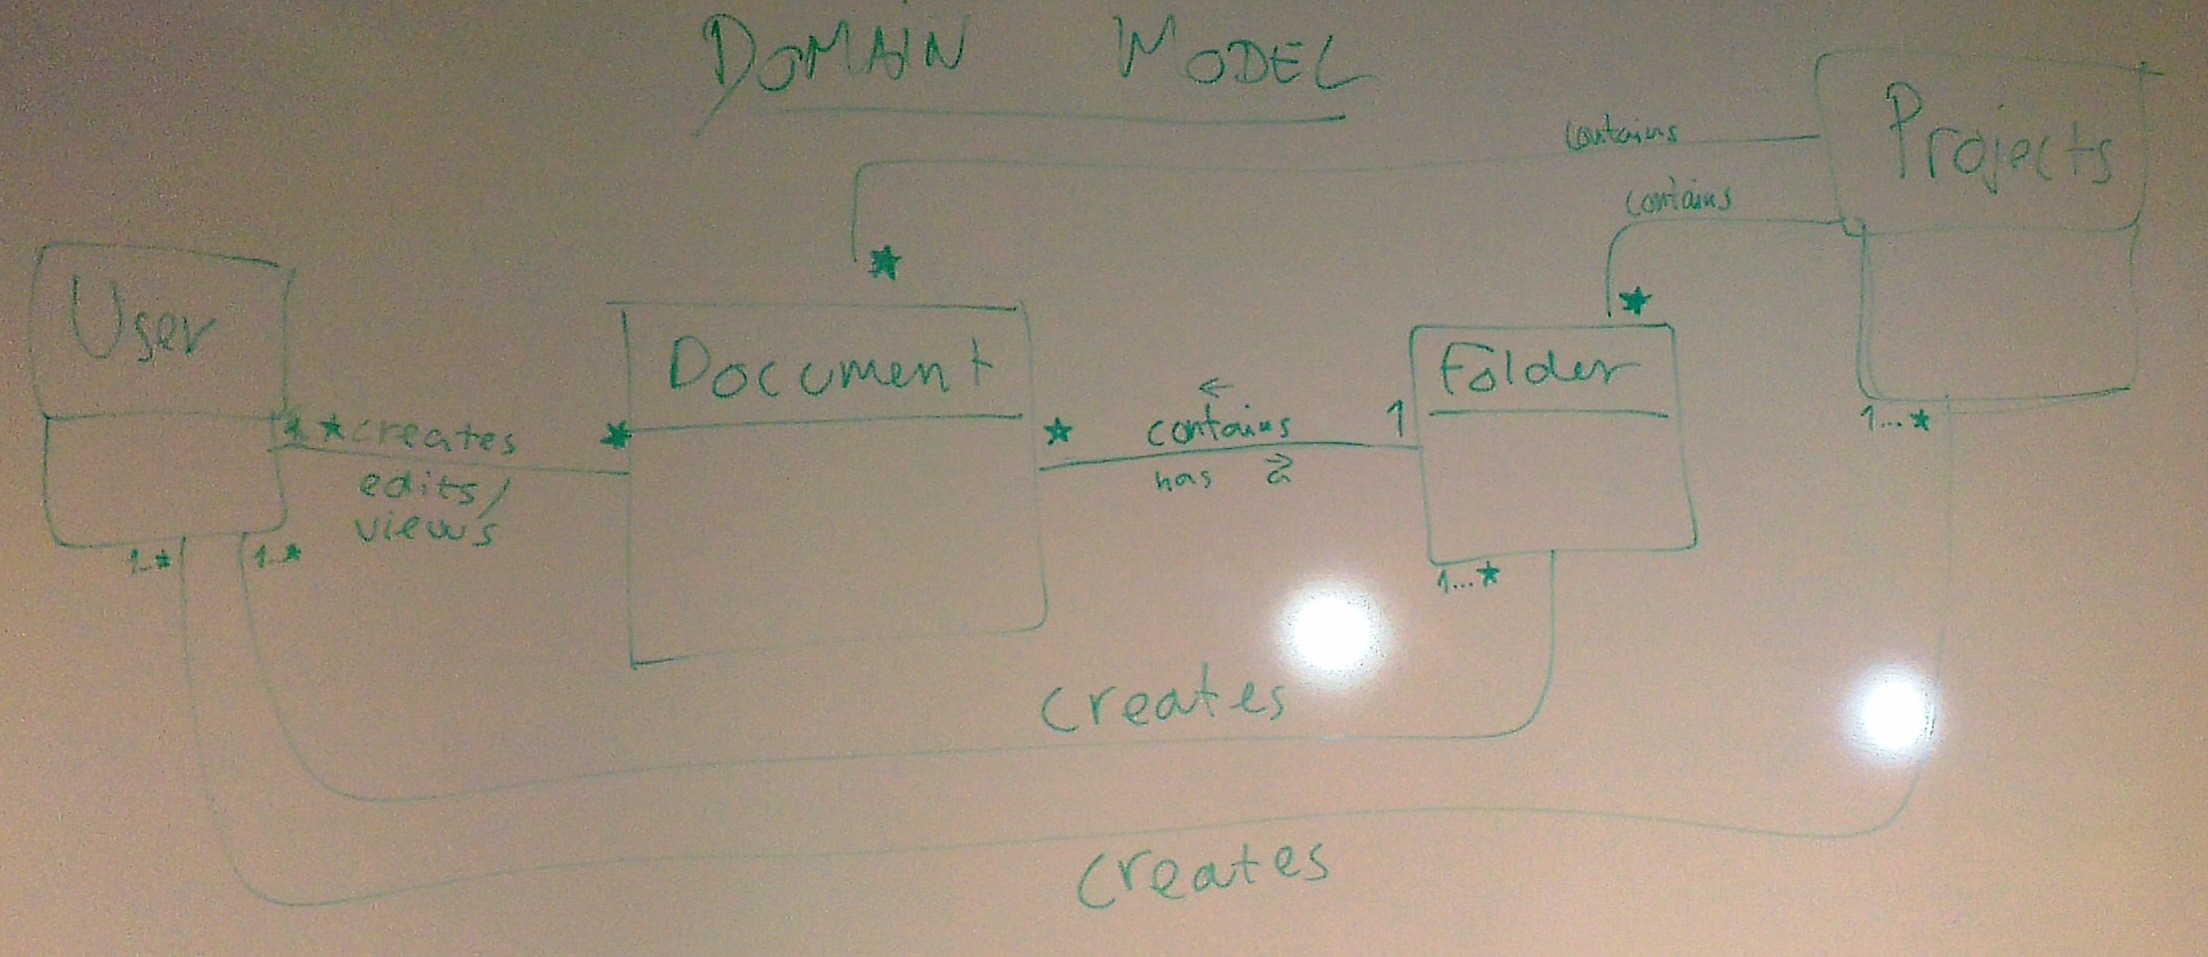
\includegraphics[width=\textwidth,natwidth=2208,natheight=957]{illustrations/DomainModel.jpg}
  \caption{Domain Model}
  \label{domainmodel}
\end{figure}
The picture shows our first draft of the domain model. It shows that our domain model reflects the entities needed to fulfill the requirements given in the project description.\\
Additionally, we quickly identify that online storage using a database will be an important part of our system. As a consequence we also add a relational data model to create a better view of the entities in this aspect:\\
\begin{figure}[H]
  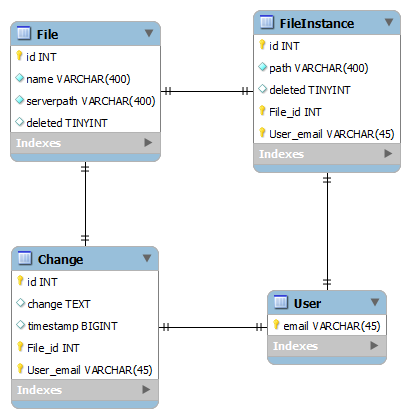
\includegraphics[width=\textwidth,natwidth=410,natheight=418]{illustrations/RelationalData-model.png}
  \caption{Relational Data-Model}
  \label{relationalmodel}
\end{figure}
As it clearly shows, both of these models were quickly drawn and used primarily for their discussion value. The relational model also covers changes made to a document, which we did not include in the initial domain model.\\
Later, we will review both models as they are expanded to support the requirements.\\
\subsubsection{Requirements Analysis with Use Cases}
Before analyzing any requirements, a reasonable exercise could be to create a vision for the product to develop \cite[p.~58]{OOAD}. However, as the high level requirements were already defined in the project description, we decide to skip this artifact.\\
\newline
Understanding the requirements means creating different artifacts that helps develop early ideas of how to solve each requirement. We write down several use cases in a brief form, only covering 1) the goal of the use case and 2) brief explanations of scenarios. A few of the use cases are expanded to include an extended description of alternate case flows as well as pre- and postconditions. Below is an example of a brief use case, ViewVersionHistory:\\
\newline
% [UseCase #4 here in cursive as a quote and delete it from appendix].  
\texttt{USE CASE \#4: VIEW VERSION HISTORY\\
The user wants to view a history for a file in the Slice Of Pie system. He will select a file from the graphical user interface in the system and click on a show version history button. The system will retrieve version history for the file and display it in a new window. \\
ALTERNATE:\\
The user wants to revert document to an earlier state. This use case has yet to be defined and elaborated on.}\\
% Margin?
\newline
The example shows a Use Case detailing the process of viewing a version history of a file.
The use cases created in this sprint are shown in [Appendix, Use Cases page \pageref{usecases}].
% ref
\subsubsection{Non-trivial requirements}
To further elaborate on requirements that may require complex implementation in the system, we create additional artifacts to understand them. The example we will show here is the users ability to synchronize documents between a client and the server holding the documents in online storage. To illustrate the interaction between the user and the system when this process is occurring, a System Sequence Diagram is drawn to display this [Appendix, Illustrations, Figur \ref{activitydiagram}, \pageref{systemsequencediagram}]. The SSD is shown in the Appendix.\\
Moreover, to elaborate on the conditions of the requirement, we create an Operation Contract as shown below:\\
\begin{table*}[ht]\centering
  \ra{1.3}
  \begin{tabularx}{\textwidth}{@{}rXXl@{}}\toprule
    \textbf{Contract CO1:} & SynchronizeWithServer\\
    \textbf{Cross References:} & Use Case \#2: Synchronize\\
    \textbf{Preconditions:} &  The user has an internet connection. The server is up and running.\\
    \textbf{Postconditions:} & The user has received files made in another client application.\\
    & The client has sent files to online storage.\\
    & The user interface displays the newly received files.\\
    \bottomrule
  \end{tabularx}
\end{table*}
The artifacts described above serves to make the requirement explicit and well-defined. The requirement is purely functional, however, and does not specify any measurable quality factors on the Use Case such as: how fast the process should be, how we should handle errors etc. However, trying to elaborate on all requirements is a time-consuming process and as RUP suggests \cite[12.2 p.~196]{OOAD}, we will instead start implementing the high-risk elements of the requirements, then review and adapt the requirements at a later iteration. \\
\subsubsection{Supplementary Specification}
As part of the initial analysis, it is suggested by RUP that a coarse supplementary specification is started in the inception of the iterative development \cite[7.1 p.~102]{OOAD}. Hence, we create an outline of the non-functional requirements in a Supplementary Specification. The non-functional requirement is presented as the FURPS+ checklist. The main reason for this specification is the impact the non-functional requirements may have on the logical architecture of the system.\\
\newline
The Supplementary Specification concludes our artifacts created as part of the initial analysis. These artifacts are mainly supposed to provide a base for our initial code design and choice of logical architecture.\\
\subsection{Initial Design and Architecture}
This section covers our initial program design. We will show the artifacts related to the process of choosing a logical architecture and their influence. Moreover, we'll describe and discuss Class Diagrams as our layers in our architecture were initially thought out. 
% [maybe we need some more introduction here]
\subsubsection{Logical Architectural Design}
% refs following
Our initial logical architectural design signals a transition from understanding and analysing the requirements to actually outlining major subsystems of the program. This is done with the artifacts from earlier described in mind.\\
The requirements explicitly state that the program should contain two modes of program execution: offline and online work. Hence, in order to use several features of the .NET framework we decide to make separate User Interfaces to support this. It follows that we need some separation between UI and the logic applied when synchronizing documents between applications as according to the Model-View separation Principle \cite[p.~209]{OOAD}. Additionally, we want to introduce a layer between persistence of the documents and the synchronization logic specific to the client or the server. Outlining this initial architecture is a very crude UML package diagram as shown in [Appendix, Figur \ref{packagediagram}, page \pageref{packagediagram}].
% or maybe a minimized version]. 
% ref
The package diagram shows separate subsystems, but in a logical partition. This means we may implement packages such as GUI(Web) and GUI(Offline) in separate applications.\\
As we will show later, the architecture shown in the diagram needs some improvement, which we do in the next iteration. The argument for this decision is that we want to identify and implement a core solution for the critical elements of the program such as persisting files, marshalling files and synchronizing files (as early as possible in development).\\
\subsubsection{Initial Client Server Class Design}
This section describes an overview of our class design as we envision it during the first sprint. Based on the Synchronization use case, U\#2, we realize the need for a central entity responsible for synchronizing data between possible multiple clients. We decide on a basic server-client pattern divided into three tiers. The pattern contains the following characteristics:\\
\begin{itemize}
\item It allows for multiple clients to access remote storage independently.
\item It splits a potential fat client up into a thinner client and a domain server, which apply logic for example specific to synchronizing between users
\item A front-end client need only concentrate on it's own responsibilities such as - document editing and local persistence \cite{ttda}\\.
\end{itemize}
These traits allows us to build a proof-of-concept that contains the minimum requirements. Additionally, the proof-of-concept is expandable to contain for example a client written in another language. On the other hand, it contains some more implementation. Moreover, we need to define some interfaces early for the server and the client to implement. These initial crude designs is shown in our initial overview of the classes a server and a client could contain [Appendix, Figur \ref{classdiagramserver} and \ref{classdiagramclient}, page \pageref{classdiagramserver}].\\
% Insert picture?
These initial diagram are very flawed and incomplete, but nevertheless have a profound impact on our later design, as we shall see.\\
\newline
This concludes our first sprint and the connected artifacts. We have developed artifacts thats relevant to the inception and elaboration phase of RUP which we think were necessary to obtain three central objectives:\\
\begin{itemize}
\item to create a common terminology and understanding of the domain which we are required to work in
\item to analyse and interpret the requirements and their implications on the system architecture
\item to identify critical elements of our system and start implementing them.
\end{itemize}
Several of the artifacts will be revisited later as they serve different functions during the sprint.\\
% Add figures
\section{Database Design}
We use a database on our server, to keep track of who owns which files, who has access and who made what changes to them.\\
Our relational database contains eight tables:\\
\textbf{User} describes a user. Email is used as primary key\\
\textbf{File} describes a file on the server. We use serverpath to describe the path to the folder where the file is located, and name as file name. We don't keep track of folders. By specifying the path to the folder of the file, describing folders become unnecessary. Only downside is that we are unable to handle empty folders as an empty folder is not described by any files.\\
\textbf{FileMetaData} holds meta date for a file such as resolution for pictures.\\
\textbf{FileInstance} is a relation between User and File. This describes the local path for a specific user, which allows different users to store their copy of a file, in different locations.\\
\textbf{Change} is used to keep track of who changed what in which file at what time.\\
\textbf{Project} holds the title of the project.\\
\textbf{ProjectHasFile} keeps track of which files a project references.\\
\textbf{UserHasProject} keeps track of which projects a user has.\\
\newpage